\chapter{Optimization and Resampling Algorithms} \label{chp:optimization}
\epigraph{Great quote.}{Author}
\begin{figure}[H]
	\centering
	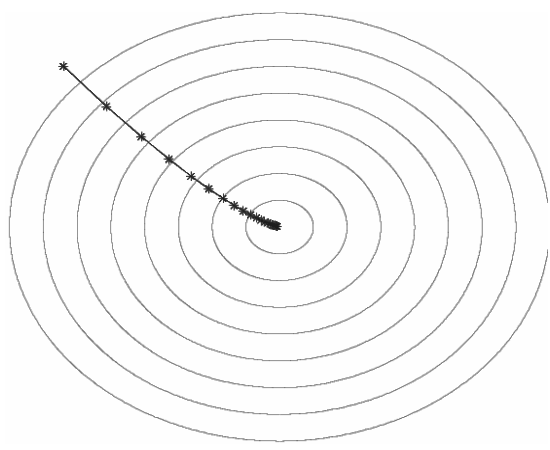
\includegraphics[scale=0.5]{Images/gd_bw.png}
	\caption{An iterative optimization algorithm is always approaching an extremum in a possibly multi-dimensional space. Here illustrated in a two-dimensional space where the equipotential curves are drawn.}
\end{figure}

In this chapter, we will cover the remaining algorithms we need before we can move on to the implementation. A good optimization algorithm is a must, we need an algorithm which can treat a large number of parameters because of the restricted Boltzmann machines. For that reason, we will introduce the ADAM optimizer, which has gained an extreme popularity after is was presented in 2014.  We also need an algorithm 

\newpage
\section{Optimization algorithms}
In chapter \ref{chp:machinelearning}, we discussed the gradient descent optimization algorithm, which is among the most basic methods available. That method is based on the gradient, which is the slope of the cost function, but many methods are also in need of the Hessian matrix, which gives the curvature of the cost function. We will overlineely scratch the surface of this field, limiting us to the gradient methods. 

To have the method fresh in mind, we will start with reintroducing the gradient descent method before we move on the its stochastic brother. We will then have a look at how momentum can be added, and finally we examine the stochastic and momentum based ADAM optimizer. 

\subsection{Gradient descent} \label{sec:gd}
Perhaps the simplest and most intuitive method for finding the minimum is the gradient descent method, which reads
\begin{empheq}[box={\mybluebox[5pt]}]{align}
\label{eq:GD}
\bs{\theta}_t=\bs{\theta}_{t-1} - \eta\nabla_{\theta} \mathcal{C}(\bs{\theta}_{t-1})
\end{empheq}
where $\bs{\theta}_t$ is the parameter vector at time step (iteration) $t$ and $\eta$ is the learning rate. $\nabla_{\theta} \mathcal{C}(\bs{\theta}_{t-1})$ is the gradient of the cost function with respect to all the parameters $\theta$ at time $t-1$. 

The idea is to find the direction where the cost function $\mathcal{C}(\bs{\theta})$ has the steepest slope, and move in the direction which minimizes the cost function. For every time step, the cost function is thus minimized, and when the gradient approaches zero the minimum is found. A possible, but basic, stop criterion is
\begin{equation}
\nabla_{\theta} \mathcal{C}(\bs{\theta}_t)<\varepsilon.
\end{equation}
where $\varepsilon$ is a tolerance. More robust methods are based on comparing the value of the cost function for several past iterations. 

In cases where the cost function is not strictly decreasing, we will have both local and global minima. Often, it is hard to say whether we are stuck in a local or global minimum, and this is where the stochasticity enters the game.

\subsection{Stochastic gradient descent}\label{sec:sgd}
Stochastic gradient descent is closely related to the gradient descent method, but the method uses randomly selected batches to evaluate the gradients, hence the stochasticity. By introducing this randomness, the parameters will not always be updated in order to minimize the energy, which makes us less likely to be stuck in a local minimum.

In practice, one splits the data set in $n$ batches, and select one of them to be used in the parameter update. Our hope is that this batch is representative for the entire data set, such that the new parameters gives a lower cost function. If that is the case, we have reduced the cost of an iteration significantly, since we only need to care about a batch. After each batch in the data set has had an opportunity to update the internal parameters, we say that we have went through an \textit{epoch}.

We are not guaranteed that updating the parameters with respect to a batch gives a lower cost function, and when it is not, we need to run more batches in order to minimize the cost function. Since each iteration is faster than for standard gradient descent, this is acceptable. As long as the batch is slightly representative for the entire data set, the cost function will be minimized in the end.

Mathematically, the method can be expressed as 
\begin{empheq}[box={\mybluebox[5pt]}]{align}
\label{eq:SGD}
\bs{\theta}_t=\bs{\theta}_{t-1} - \eta\nabla_{\theta} \mathcal{C}_i(\bs{\theta}_{t-1})
\end{empheq}
where we use the $i$'th batch in the parameter update. Standard gradient descent is actually just a special case of this, where we only have one batch ($i$ includes the whole data set). If we still get stuck in local minima after adding the stochasticity, it might be a good idea to add momentum as well.

\subsection{Adding momentum} \label{sec:momentum}
If we go back to an introductory mechanics course, you might remember that momentum is a quantity that maintains the motion of a body. Imagine a ball that rolls down a steep hill, but then there is a local minimum that it needs to escape to keep rolling. If it has enough momentum, it will be able to escape.

Exactly the same idea lies behind the momentum used in optimization algorithms; the momentum will try to maintain the motion towards the global minimum, which makes the system less likely to be stuck in a local minimum.  

Momentum can be added to most optimization algorithms, also gradient descent and stochastic gradient descent. The way we do it is to save the direction we were moving in the previous iteration, and use it as a contribution to the next gradient update. A typical implementation of the first-order momentum looks like
\begin{empheq}[box={\mybluebox[5pt]}]{equation}
\begin{aligned}
\bs{m}_t &= \gamma\bs{m}_{t-1} + \eta\nabla_{\theta} \mathcal{C}_i(\bs{\theta}_{t-1})\\
\bs{\theta}_t&=\bs{\theta}_{t-1}-\bs{m}_t
\end{aligned}
\end{empheq}
where $\gamma$ is the momentum parameter, which is just another hyper-parameter usually initialized to a small number. $\bs{m}_t$ is the momentum vector, and can be initialized as the zero vector.

The optimization algorithm can be modified further in unlimited ways. A common improvement is to add higher order momentum, another is to make the learning rate adaptive. We have implemented the most basic version of this, with monotonic adaptivity. Many algorithms, such as the conjugate gradient method, also make use of the Hessian as discussed in the introduction, but that is another level of complexity. 

We will end this section with setting up the algorithm of a stochastic gradient descent optimization with momentum and monotonic adaptivity. The algorithm is found in algorithm \eqref{alg:asgd}.

\IncMargin{1em}
\begin{algorithm}
	\SetAlgoLined
	\Parameter{$\eta$: Learning rate}
	\Parameter{$\gamma$: Momentum parameter}
	\Parameter{$\lambda$: Monotonic decay rate}
	\Require{$\mathcal{C}(\bs{\theta})$: Cost function}
	\Data{$\bs{\theta}_0$: Initial parameters}
	
	$\bs{m}_0\leftarrow 0$ (Initialize momentum vector)\;
	$t\leftarrow 0$ (Initialize time step)\;
	\While{$\bs{\theta}_t$ not converged}{
		$t\leftarrow t+1$ (Increase time for each iteration)\;
		$\bs{g}_t\leftarrow \nabla_{\theta}\mathcal{C}_t(\bs{\theta}_{t-1})$ (Get gradients from a given batch at time $t$)\;
		$\bs{m}_t\leftarrow \gamma\bs{m}_{t-1}+\eta\cdot\bs{g}_t$ (Update first momentum estimate)\;
		$\bs{\theta}_t=\bs{\theta}_{t-1}-\eta\cdot\bs{m}_t/\lambda^t$ (Update parameters)\;
	}
	\KwResult{Updated parameters $\bs{\theta}_t$ after convergence}
	\caption{Adaptive stochastic gradient descent with momentum. See sections (\ref{sec:sgd}-\ref{sec:momentum}) for details. Robust default settings for the hyper-parameters are $\eta=0.001$, $\gamma=0.01$ and $\lambda=0.1$. All the operations are element-wise.}
	\label{alg:asgd}
\end{algorithm}\DecMargin{1em}

\subsection{ADAM}
ADAM is a first-order stochastic optimization method which is widely used in machine learning. It was discovered by D.P. Kingma and J. Ba, and published in a 2014 paper. The article has already more than 25000 citations! \cite{kingma_adam:_2014} So what makes this method so popular? 

The main reason why it is widely used, is obviously that it performs good. The fact that it only requires the gradient makes it efficient, and the way the momentum is implemented still makes able to handle a large number of parameters. 

The optimization algorithm can be expressed as a set of equations
\begin{empheq}[box={\mybluebox[5pt]}]{equation}
\begin{aligned}
\bs{g}_t&=\nabla_{\theta} \mathcal{C}_t(\bs{\theta}_{t-1})\\
\bs{m}_t&=\gamma_1\bs{m}_{t-1}+(1-\gamma_1)\bs{g}_t\\
\bs{v}_t&=\gamma_2\bs{v}_{t-1}+(1-\gamma_2)\bs{g}_t^2\\
\hat{\bs{m}}_t&=\bs{m}_t/(1-\gamma_1^t)\\
\hat{\bs{v}}_t&=\bs{v}_t/(1-\gamma_2^t)\\
\bs{\theta}_t&=\bs{\theta}_{t-1}-\eta\hat{\bs{m}}_t/(\sqrt{\hat{\bs{v}}_t}+\bs{\varepsilon})
\end{aligned}
\end{empheq}
where $\bs{m}_t$ is the biased first momentum estimate of the parameter vector $\bs{\theta}$ and $\bs{v}_t$ is the biased second raw moment estimate. The momentum parameters need to be in the range $\gamma_1,\gamma_2\in[0,1)$, and are often set to values close to 1. This makes the optimization adaptive: as time goes, the factors $1-\gamma_1^t$ and $1-\gamma_2^t$ approach 1 from below. $\eta$ corresponds to the learning rate, and should be a small number. Finally, the parameter $\varepsilon$ is added to avoid division by zero. 

We can set up the algorithm in a similar manner to the adaptive stochastic gradient descent algorithm from above, which gives the algorithm \eqref{alg:adam}.

\IncMargin{1em}
\begin{algorithm}
	\SetAlgoLined
	\Parameter{$\eta$: Learning rate}
	\Parameter{$\gamma_1,\gamma_2\in [0,1)$: Momentum parameters}
	\Parameter{$\varepsilon$: Division parameter}
	\Require{$\mathcal{C}(\bs{\theta})$: Cost function}
	\Data{$\bs{\theta}_0$: Initial parameters}
	
	$\bs{m}_0\leftarrow 0$ (Initialize 1$^{\text{st}}$ momentum vector)\;
	$\bs{v}_0\leftarrow 0$ (Initialize 2$^{\text{st}}$ momentum vector)\;
	$t\leftarrow 0$ (Initialize time step)\;
	\While{$\bs{\theta}_t$ not converged}{
		$t\leftarrow t+1$ (Increase time for each iteration)\;
		$\bs{g}_t\leftarrow \nabla_{\theta}\mathcal{C}_t(\bs{\theta}_{t-1})$ (Get gradients from a given batch at time $t$)\;
		$\bs{m}_t\leftarrow \gamma_1\bs{m}_{t-1}+(1-\gamma_1)\cdot\bs{g}_t$ (Update first momentum estimate)\;
		$\bs{v}_t\leftarrow \gamma_2\bs{v}_{t-1}+(1-\gamma_2)\cdot\bs{g}_t^2$ (Update second raw momentum estimate)\;
		$\hat{\bs{m}}_t\leftarrow\bs{m}_t/(1-\gamma_1^t)$ (Bias-corrected first momentum estimate)\;
		$\hat{\bs{v}}_t\leftarrow\bs{v}_t/(1-\gamma_2^t)$ (Bias-corrected second momentum estimate) \;
		$\bs{\theta}_t\leftarrow\bs{\theta}_{t-1}-\eta\cdot\hat{\bs{m}}_t/(\sqrt{\hat{\bs{v}}_t}+\bs{\varepsilon})$ (Update parameters) \;
	}
	\KwResult{Updated parameters $\bs{\theta}_t$ after convergence}
	\caption{ADAM optimizer. Robust default settings for the hyper-parameters are $\eta=0.001$, $\gamma=0.01$ and $\lambda=0.1$. All the operations are element-wise, and for in-depth information see the original paper, \cite{kingma_adam:_2014}.}
	\label{alg:adam}
\end{algorithm}\DecMargin{1em}

\section{Variance estimation} \label{sec:variance}
In experiments, we have two main classes of errors, systematical errors and statistical errors. The former is a result of external factors such as uncertainties in the apparatus or a person constantly takes an incorrect measurement, which is an error that is hard to estimate. The latter, however, can be found by estimating the variance of the sample mean, which we want to find accurate and efficient. Monte-Carlo simulations can be treated as computer experiments, and therefore we can use the same analyzing tools as we do for real experiments. 

There are several ways to estimate the variance, where the cheapest ones also are the less accurate ones. To make the most use of our data, we use resampling methods to estimate the statistical errors. Some well-known resampling algorithms are blocking, bootstrap and jackknife. We will cover the blocking method only, since that is the only one we use in our particular implementations. To save computational time, we resample the final iteration only, for the others we use the simple estimation method.

\subsection{Basic concepts of statistics}
Before we go through the methods, we will give a brief introduction to some useful statistical quantities. We start with the \textit{moments}, which are given by
\begin{equation*}
\langle x^n\rangle=\int dxp(x)x^n
\end{equation*}
where $p(x)$ is the true \textit{probability density function}. In order to make physical sense, this function needs to normalized such that the integral over all possible outcomes gives a total probability of 1. This is the zero'th moment, $\int dxp(x)=1$. The first moment is the \textit{mean} of $p(x)$, and is often denoted by the letter $\mu$
\begin{equation}
\langle x\rangle=\mu=\int dxp(x)x
\end{equation}
Furthermore, we can define the \textit{central moments} given by
\begin{equation}
\langle(x-\langle x\rangle)^n\rangle=\int dx(x-\langle x\rangle)^np(x),
\end{equation}
which is centered around the mean. With $n=0$ and $n=1$, this is easy to find, but what is the central moment with $n=2$? The central moment with $n=2$ is what we call the \textit{variance}, and is often denoted as $\sigma^2$ as we did in the equation \eqref{eq:variance}. One can show that
\begin{equation}
\sigma^2=\langle(x-\langle x\rangle)^2\rangle=\langle x^2\rangle - \langle x \rangle^2
\label{eq:variance2}
\end{equation}
which was already stated in the theory chapter. The \textit{standard deviation} is given by the square-root of the variance, $\sigma$, and is the quantity we will present as the measure of the uncertainty in the last digit of a numerical result. 

Using the expressions above, we can calculate the mean and the variance of a probability density function $p(x)$, but what do we do if we have a set of data drawn from an unknown $p(x)$?

If the probability density function is unavailable, we cannot find the exact sample mean and sample mean variance. However, we can make an estimate, writing
\begin{equation}
\langle X\rangle\approx \frac{1}{n}\sum_{i=1}^n X_i\equiv\overline{X},
\end{equation}
for the sample mean assuming that $X$ is our sample containing $n$ points. Further, the variance of the sample mean, assuming that the measurements are \textit{independent}, can be found from
\begin{equation}
\text{var}(\overline{X})\equiv\frac{1}{n}\sum_{i=1}^n(X_i-\overline{X})^2=\frac{\sigma^2}{n}
\label{eq:samplevariance}
\end{equation}
where $\sigma^2$ is the variance of the probability density function. The law of large numbers states that the estimated sample mean approaches the true sample mean as $n$ goes to infinity. This is closely related to the central limit theorem, which says that the probability distribution of $X$, $p_X(x)$, can be approximated as a normal distribution with $\mu=\overline{X}_n$ and $\sigma=\text{var}(\overline{X})$ as the number of sampling points $n$ goes to infinity. 

On the other hand, if the samples are \textit{correlated}, equation \eqref{eq:samplevariance} becomes an underestimation of the \textit{sample error} $\text{err}_X^2$, and is thus more a guideline for the size of the uncertainty, more than an actual estimate of it. In that case, we need to calculate the more general \textit{covariance}, given by 
\begin{equation}
\text{cov}(X_i,X_j)=(X_i-\overline{X})(X_j-\overline{X})
\end{equation}
which gives a measure on the correlations between $X_i$ and $X_j$. Note that the variance is just the special case where $X_i$ and $X_j$ are independent. We define the sample error as
\begin{equation}
\text{err}_{X}^2=\frac{1}{n^2}\sum_{i=1}^n\sum_{j=1}^n\text{cov}(X_i,X_j)
\end{equation}
which can be further expressed as a function of the \textit{autocovariance}, defined as 
\begin{equation}
\gamma(h)=\text{cov}(X_i,X_{i+h})
\end{equation}
and is thus just a measure of the correlation of a part of a time series with another part of the same time series. If $h=0$, this is just the variance, $\gamma(h)=\sigma^2$. Using this, the sample error reads
\begin{equation}
\text{err}_X^2=\frac{\sigma^2}{n}+\frac{2}{n}\sum_{h=1}^{n-1}\Big(1-\frac{h}{n}\Big)\gamma(h).
\label{eq:samplevariance2}
\end{equation}

A problem with this definition of the sample error, is that it turns out to be very expensive to calculate as the number of samples gets large. We are in need of a cheaper method, which is the task of the resampling methods. We will in the following discuss the blocking algorithm, which is the resampling method of choice in this work. 

\subsection{Blocking}\label{sec:resampling}
Above, we have described the need of a proper estimation of the uncertainty in computational simulations, where the covariance was included in
the calculation of $\sigma^2$. A quick and easy way to get a proper estimate of the uncertainty, is by using the blocking method.

When the blocking method was made popular by Flyvberg and Peterson in 1989, the method required hyper-parameters which had to be carefully adjusted for each particular data set. \cite{flyvbjerg_error_1989} In 2018, Marius Jonsson reinvented the algorithm and made it automated, with no need for external parameters. Despite this, no compromise was made on performance. The method scales as $12n+\mathcal{O}(\log_2n)$ for small data sets, but reduces to $n+\mathcal{O}(1)$ for large data sets, which makes it preferred over bootstrap and jackknife for large data sets. \cite{jonsson_standard_2018} We will now go through the idea behind the blocking method.

Consider a time series $\{x_1, x_2, \hdots, x_n\}$ with $n=2^d$ data point for some integer $d>1$. For this series, an autocovariance function $\gamma(h)$ is guaranteed to exist. We arrange the data in a vector
\begin{equation}
X=(x_i,x_2,\hdots,x_n),
\end{equation}
which we assume to be asymptotically uncorrelated. The idea is to take the mean of subsequent pair of elements from $X$, and form a new vector $X_1$. We then repeat the operation on $X_1$ and form a new vector $X_2$ and so on. This is the reason why we require $n=2^d$. If $k$ denotes an element in vector $X_i$, we can write the procedure recursively as
\begin{equation}
\begin{aligned}
(X_0)_k&\equiv(X)_k\\
(X_{i+1})_k&\equiv\frac{1}{2}\Big((X_i)_{2k-1}+(X_i)_{2k}\Big)
\end{aligned}
\end{equation}
where $1\leq i\leq d-1$ and $1\leq k\leq n/2^i$, which are known as the \textit{blocking transformations}. According to equation \eqref{eq:samplevariance2}, we can express the sample mean variance of $X_k$ as
\begin{equation}
\text{var}(\overline{X}_k)=\frac{\sigma_k^2}{n_k}+\frac{2}{n_k}\sum_{h=1}^{n_k-1}\Big(1-\frac{h}{n_k}\Big)\gamma_k(h),
\end{equation}
where we define the last term as the \textit{truncation error}, $e_k$, as it is intractable. It can be shown that the sample variance of all pairs $(X_i)_k$ and $(X_j)_k$ after a while will be identical \cite{flyvbjerg_error_1989},
\begin{equation}
\text{var}(\overline{X}_i)=\text{var}(\overline{X}_j)
\label{eq:varivarj}
\end{equation}
with the consequence that the sample mean variance of the entire set of samples if also given by
\begin{equation}
\text{var}(\overline{X})=\frac{\sigma_k^2}{n_k}+e_k\quad\quad\forall\quad 0\leq k\leq d-1.
\end{equation}
In the original (manual) blocking method, we had to know exactly where to stop the procedure in order to equation \eqref{eq:varivarj} to hold. If we do not continue long enough, the sample variance has not converged, while if we keep on going for too long, the standard error of $\text{var}(\hat{\sigma}_k^2/n_k)$ get very large. If one plots the sample variance as a function of the iterations, one will see that the curve forms a plateau before it gets very noisy, but with Jonsson's automated method, we do not need to worry about this. 

We will end this section by scratching the most basic blocking algorithm

\IncMargin{1em}
\begin{algorithm}
	\SetAlgoLined
	\Data{$\bs{X}$: Initial samples}
	\BlankLine
	$\bs{X}_0\leftarrow \bs{X}$ (Redefine initial data set)\;
	$i\leftarrow 0$ (Initialize step)\;
	\While{$\text{var}(\bs{X}_{i+1})\neq \text{var}(\bs{X}_{i})$}{
		$n_i\leftarrow n/2^i$ (Number of elements in $\bs{X}_i$)\;
		$\text{var}(\bs{X}_i)\leftarrow\sigma_i^2/n_i$ (Estimate the variance of $\bs{X}_i$)\;
		\For{$k\leftarrow 1$ \KwTo $n_i$}{
			$(\bs{X}_{i+1})_k\leftarrow0.5\big((\bs{X}_i)_{2k-1}+(\bs{X}_i)_{2k}\big)$ (The blocking transformations)\;
		}
		$i\leftarrow i+1$ (Increase $i$ for each iteration)\;
	}
	\KwResult{The sample mean variance of the initial data set $\bs{X}$.}
	\caption{Sketch of the blocking method. Here we find the sample mean variance of the data set $\bs{X}$ containing $n$ samples. See section \ref{sec:variance} for details.}
	\label{alg:blocking}
\end{algorithm}\DecMargin{1em}

In our work, we will consequently use Marius Jonsson's automated blocking algorithm and code, available on \url{https://github.com/computative/block}.

\section{Summary of the algorithms}
Up to this point we have presented several algorithms that contribute to the variational Monte-Carlo algorithm, and to give the reader a complete description of the simulating procedure, we will here summarize them and place them in the correct order. First, Metropolis-Hastings algorithm was given, which is responsible for the sampling. Thereafter, we presented a few optimization algorithms, before the blocking algorithm was given. 

The optimization loop forms the outer environment, 

\IncMargin{1em}
\begin{algorithm}
	\SetAlgoLined
	
	\Parameter{$\eta$: Learning rate}
	\Parameter{$\Delta x$: Step length}
	\Require{$\Psi_T(\bs{r},\bs{\theta})$: Trial wave function}
	\BlankLine
	$\bs{r}\leftarrow \mathcal{N}(0,\sigma^2)$ (Initialize positions randomly)\;
	$\bs{\theta}\leftarrow \mathcal{U}(0,1)$ (Initialize parameters, could be randomly)\;
	\While{not converged}{ 
		$\bs{E}\leftarrow[-]$ (Declare an empty local energy list)\;
		$\bs{d}_{\theta}\leftarrow[-]$ (Declare an empty parameter gradient list)\;
		$\bs{Ed}_{\theta}\leftarrow[-]$ (Declare an empty list containing parameter gradient $\cdot$ local energy)\;
		\For{$i\leftarrow 1$ \KwTo $M$}{
			$\bs{r}\leftarrow\bs{r}+\Delta x$ (Update position)\;
			\If{$\Psi_T(\bs{r}_{\text{new}})/\Psi_T(\bs{r}_{\text{old}})<\mathcal{U}(0,1)$}{
				reject move \;
			}
			$E^i\leftarrow \big(\hat{\mathcal{H}}\Psi_T(\bs{r},\bs{\theta})\big)/\Psi_T(\bs{r},\bs{\theta})$ (Fill $\bs{E}$-list with local energies) \;
			$d_{\theta}^i\leftarrow \nabla_{\theta}\ln\Psi_T(\bs{r})$ (Fill $\bs{d}_{\theta}$-list with parameter gradients) \;
			$Ed_{\theta}^i\leftarrow \bs{E}^i\cdot\bs{d}_{\theta}^i$ (Fill $\bs{Ed}_{\theta}$-list) \;
		}
		$\bs{E}_0\leftarrow \bs{E}$\;
		$i\leftarrow 0$ (Initial blocking step)\;
		\While{$\text{var}(\bs{E}_{i+1})\neq \text{var}(\bs{E}_{i})$}{
			$n_i\leftarrow n/2^i$ (Number of elements in $\bs{E}_i$)\;
			$\text{var}(\bs{E}_i)\leftarrow\sigma_i^2/n_i$ (Estimate the variance of $\bs{E}_i$)\;
			\For{$k\leftarrow 1$ \KwTo $n_i$}{
				$(\bs{E}_{i+1})_k\leftarrow0.5\big((\bs{E}_i)_{2k-1}+(\bs{E}_i)_{2k}\big)$ (The blocking transformations)\;
			}
			$i\leftarrow i+1$ (Increase $i$ for each iteration)\;
		}
		$\overline{\bs{E}}\leftarrow\sum_{j=1}^ME^j/M$ (Compute the local energy sample mean)\;
		$\overline{\bs{d}}_{\theta}\leftarrow\sum_{j=1}^Md_{\theta}^j/M$ (Compute the sample mean of $\bs{d}_{\theta}$)\;
		$\overline{\bs{Ed}}_{\theta}\leftarrow\sum_{j=1}^MEd_{\theta}^j/M$ (Compute the sample mean of $\bs{Ed}_{\theta}$)\;
		$G_{\theta}\leftarrow2\big(\overline{\bs{Ed}}_{\theta}-\overline{\bs{E}}\cdot\overline{\bs{d}}_{\theta}\big)$\;
		$\bs{\theta}\leftarrow \bs{\theta}-\eta\cdot G_{\theta}$\;
	}
	\KwResult{An estimate of the many-body wave function $\Psi(\bs{r})$ and the local energy $\langle E_L\rangle\approx\overline{\bs{E}}$ with its uncertainty $\text{var}(\overline{\bs{E}})$.}
	\caption{The variational Monte-Carlo algorithm in its simplest form. The outer loop is for the parameter update. The first inner loop is the sampling where $M$ is the number of Monte-Carlo cycles, and the last inner loop is the resampling loop. Note that we present the brute-force Metropolis algorithm, while the more robust Metropolis-Hasting algorithm, found in algorithm \ref{alg:hastings}, is preferred. Furthermore, we also limit us to the simple gradient descent method. $\mathcal{N}(\mu,\sigma)$ denotes a normal distribution with mean $\mu$ and variance $\sigma$, while $\mathcal{U}(0,1)$ denotes a uniform distribution between 0 and 1. }
	\label{alg:total}
\end{algorithm} \DecMargin{1em}







